\documentclass[tikz,border=12pt]{standalone}
\usepackage{amsmath,amssymb}
\usetikzlibrary{positioning,decorations.pathreplacing,calc,shapes.geometric,fit,arrows.meta}

\begin{document}
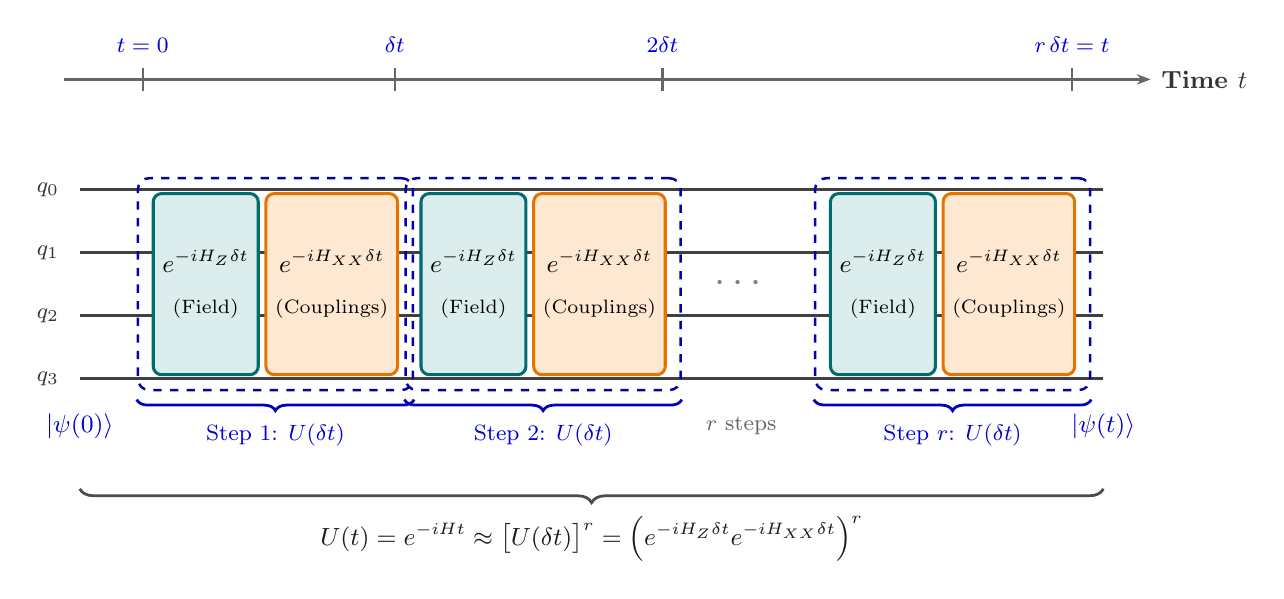
\begin{tikzpicture}[
    wire/.style={line width=1.1pt, draw=black!75},
    sublayerZ/.style={draw=teal!85!black, fill=teal!14, rounded corners=3pt, line width=1.1pt, minimum width=1.2cm, minimum height=2.3cm, font=\small, align=center},
    sublayerXX/.style={draw=orange!90!black, fill=orange!18, rounded corners=3pt, line width=1.1pt, minimum width=1.3cm, minimum height=2.3cm, font=\small, align=center},
    timenode/.style={font=\footnotesize\color{blue!85!black}},
    timeaxis/.style={line width=1.0pt, draw=black!60, -{Stealth[length=5pt]}}
]

    % Time axis along the top
    \draw[timeaxis] (-1.0, 3.4) -- (12.8, 3.4) node[right, font=\small\bfseries\color{black!80}] {Time $t$};
    \foreach \x/\txt in {0/{$t=0$}, 3.2/{$\delta t$}, 6.6/{{$2\delta t$}}, 11.8/{{$r\,\delta t = t$}}} {
        \draw[line width=0.8pt, draw=black!60] (\x, 3.25) -- (\x, 3.55);
        \node[above=2pt, timenode] at (\x, 3.55) {\txt};
    }

    % Qubit wires
    \foreach \y [count=\i from 0] in {2.0, 1.2, 0.4, -0.4} {
        \node[font=\footnotesize\color{black!80}, left=4pt] at (-0.8, \y) {$q_\i$};
        \draw[wire] (-0.8, \y) -- (12.2, \y);
    }

    % Initial state label
    \node[font=\small\color{blue!80!black}] at (-0.8, -1.0) {$|\psi(0)\rangle$};

    % --- Step 1: [0, dt] ---
    \node[sublayerZ] (z1) at (0.8, 0.8) {$e^{-i H_Z \delta t}$\\[4pt]\scriptsize (Field)};
    \node[sublayerXX] (xx1) at (2.4, 0.8) {$e^{-i H_{XX} \delta t}$\\[4pt]\scriptsize (Couplings)};
    \node[draw=blue!70!black, dashed, rounded corners=4pt, line width=0.9pt, fit=(z1)(xx1), inner sep=5pt] (step1) {};
    \draw[decorate, decoration={brace, amplitude=4pt, mirror}, line width=1.0pt, draw=blue!75!black] 
        ($(step1.south west)+(0,-3pt)$) -- ($(step1.south east)+(0,-3pt)$)
        node[midway, below=5pt, font=\footnotesize\color{blue!85!black}] {Step 1: $U(\delta t)$};

    % --- Step 2: [dt, 2dt] ---
    \node[sublayerZ] (z2) at (4.2, 0.8) {$e^{-i H_Z \delta t}$\\[4pt]\scriptsize (Field)};
    \node[sublayerXX] (xx2) at (5.8, 0.8) {$e^{-i H_{XX} \delta t}$\\[4pt]\scriptsize (Couplings)};
    \node[draw=blue!70!black, dashed, rounded corners=4pt, line width=0.9pt, fit=(z2)(xx2), inner sep=5pt] (step2) {};
    \draw[decorate, decoration={brace, amplitude=4pt, mirror}, line width=1.0pt, draw=blue!75!black] 
        ($(step2.south west)+(0,-3pt)$) -- ($(step2.south east)+(0,-3pt)$)
        node[midway, below=5pt, font=\footnotesize\color{blue!85!black}] {Step 2: $U(\delta t)$};

    % Ellipsis
    \node[font=\Large\color{black!50}] at (7.6, 0.8) {$\cdots$};
    \node[font=\footnotesize\color{black!60}] at (7.6, -1.0) {$r$ steps};

    % --- Step r: [(r-1)dt, t] ---
    \node[sublayerZ] (zr) at (9.4, 0.8) {$e^{-i H_Z \delta t}$\\[4pt]\scriptsize (Field)};
    \node[sublayerXX] (xxr) at (11.0, 0.8) {$e^{-i H_{XX} \delta t}$\\[4pt]\scriptsize (Couplings)};
    \node[draw=blue!70!black, dashed, rounded corners=4pt, line width=0.9pt, fit=(zr)(xxr), inner sep=5pt] (stepr) {};
    \draw[decorate, decoration={brace, amplitude=4pt, mirror}, line width=1.0pt, draw=blue!75!black] 
        ($(stepr.south west)+(0,-3pt)$) -- ($(stepr.south east)+(0,-3pt)$)
        node[midway, below=5pt, font=\footnotesize\color{blue!85!black}] {Step $r$: $U(\delta t)$};

    % Final state label
    \node[font=\small\color{blue!80!black}] at (12.2, -1.0) {$|\psi(t)\rangle$};

    % Overall bracket
    \draw[decorate, decoration={brace, amplitude=5pt, mirror}, line width=1.0pt, draw=black!70] 
        (-0.8, -1.8) -- (12.2, -1.8)
        node[midway, below=6pt, font=\small\color{black!90}] 
        {$U(t) = e^{-i H t} \approx \big[ U(\delta t) \big]^r = \Big( e^{-i H_Z \delta t} e^{-i H_{XX} \delta t} \Big)^r$};

\end{tikzpicture}
\end{document}
